\section{Database}

\subsection{Introduction}
One of the biggest challenges with Hatch was how to organize data. Specifically, pretty
much every organization with scientific data has their own standard or format on 
how they store research data. Many of these organizations want to share data between 
each other, but they cannot decide how to merge the formats. Consider the following
examples:

\begin{figure}[h]
	\begin{center}
	\begin{tabular}{ | c | c | c | }
		\hline
		site	&	datetime		&	unique fish tag	\\
		\hline
		TUC	&	02/16/06 19:08:15 	&	3D9.1BF1E7919A 	\\
		TUC	&	02/16/06 19:18:36 	&	3D9.1BF1A998FA 	\\
		TUC	&	02/17/06 18:21:03 	&	3D9.1BF20E8FE2	\\
		...	&	...			&	...		\\
		\hline
	\end{tabular}
	\caption{A database representing for PTAGIS data} 
	\label{ptagis_ex1}
	\end{center}
\end{figure}

\begin{figure}[h]
	\begin{center}
	\begin{tabular}{ | c | c | }
		\hline
		unique fish tag	&	DNA sequence	\\
		\hline
		3D9.1BF1E7919A 	&	ATGCTTAC...	\\
		3D9.1BF1A998FA 	&	TTACGATC...	\\
		3D9.1BF20E8FE2	&	GTGGASCT...	\\
		...		&	...		\\
		\hline
	\end{tabular}
	\caption{A database representation for DNA data} 
	\label{dna_ex1}
	\end{center}
\end{figure}

In each of the examples above, the data is represented with \textbf{rows} and 
\textbf{columns}, much the same way someone would represent the data in a Microsoft
Excel spreadsheet. These structures in a typical \textbf{relational database} (SQL, etc).
are called \textbf{tables}.

The above examples are simplifications of the rows and columns in actual research 
data. But they highlight one of the biggest issues with data storage using relational
databases: they require you to know the column names ahead of time. Not only that,
but they require that you know the data types of the values that go in those columns,
and once a table is created expecting a certain format, it is hard to change.

The problem with needing to know the structure of research data before designing
databases, is that research data \textbf{is semi-structured}, at best. Once it does
represent some structure, it often changes. For example, once researchers finally 
decide what columns and data types should go in the table in Figure \ref{ptagis_ex1},
another researcher suggests more columns that should go in to the table.

This leads to endless edits to the database and program design by some software 
developer. The standard table format that everyone can agree on isn't useful to many
researchers, because it usually leaves out a lot of other needed columns and fields.

A better approach is needed. Researchers, not committees, should decide how to store 
data. Data should be mergable based on common values in different tables (like the 
\textbf{unique fish tag} column in Figures \ref{ptagis_ex1} and \ref{dna_ex1}. The 
person who inputs the data should decide how one particular dataset is stored in a 
database, and should be able to choose to store the same data in a different table 
format, how they choose. There should be a simple tool that helps them do this.

The following sections describe different approaches to implementing a database design
that enables data storage for dynamic or semi-structured data.


\subsection{Relation Databases with table creations}
This approach is the simplest and follows the concept of table creation for data sets
pretty closely. Basically, for each input document in the form of a spreadsheet, a new
SQL table is created. The columns names and type are determined from the headers and 
data values in the spreadsheet.

\begin{figure}[h]
	\begin{center}
	\begin{lstlisting}
		CREATE TABLE ptagis_doc1
			(
				id int, 
				site char(50), 
				read_data_time date,
				tag char(50)
			); 
	\end{lstlisting}
	\caption{The SQL syntax for creating the table in Figure \ref{ptagis_ex1} } 
	\label{ptagis_ex1_sql}
	\end{center}
\end{figure}

The biggest problem with this approach with this approach is that each document
in the database is a table. When searching for a specific document, the database 
typically searches for the table name. This search is linear, and with hundreds,
thousands, or hundreds of thousands of documents, frequently searching the database
to look for values would be infinitely slow and useless.

Another problem with this design, is that building an interface like a web gui would
be difficult and complicated. 


\subsection{Relational Databases with tables for each datatype}
Another approach is to create column tables for each data type, and let document 
tables just be collections of columns. Each of the document column values point to 
respective values in the column tables.

\begin{figure}[h]
	\begin{center}
	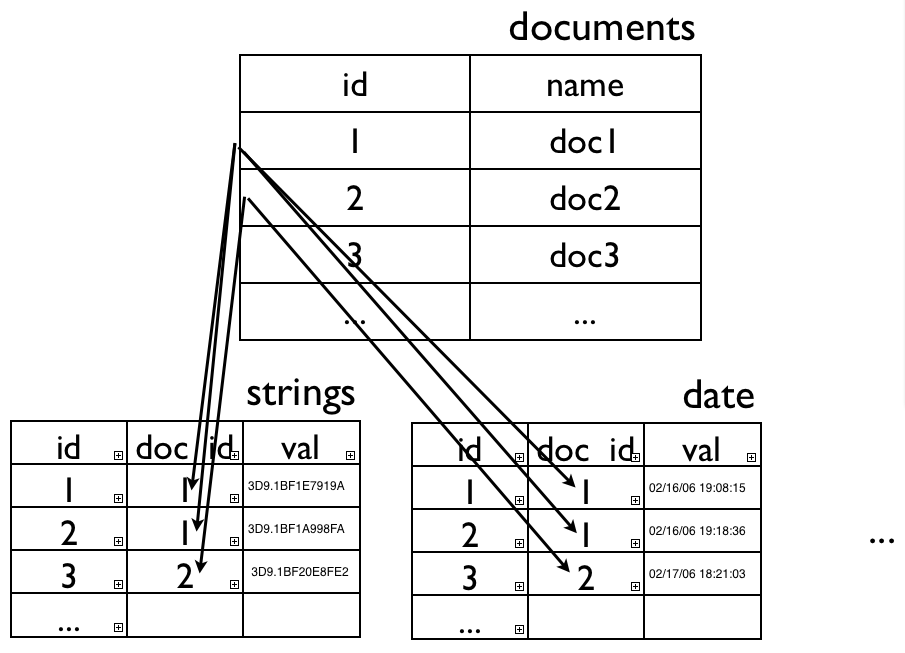
\includegraphics[width=80mm]{images/rel_db_lookup}
	\caption{Document table as a lookup table} 
	\label{rel_db_lookup}
	\end{center}
\end{figure}

This allows for documents to have a dynamic amount of columns with variable data types.
But there are two problems with this approach. First, for every value in every document
in the database, they are put into one table (i.e. all values with a 'string' data type
go into the 'string' table). With potentially millions of data values, each table
becomes an overflowing bucket, and don't utilize the the advantages of storing multiple
columns and values in one table. Searches for data would require lots of filtering 
for just the ones wanted for specific doucments, and would be inefficient.

The other issue is that every retrieval of data from a document would require lot and 
lots of lookups. Data retrieval over significantly high data sets would quickly become
very computationally intensive, and not practical.


\subsection{CouchDB}
When one thinks about the fundemental issues with storing, searching, and merging 
research data, a core issue is identified: data is semi-structured. This is what
makes trying to use relational databases so hard. They were made for datasets where
you knew the structure up front, and seldom wanted to change their structures.

The one assumption that Hatch makes about the data is that \textbf{there are rows and
columns}. This is the only assumption Hatch makes. This leaves the database and 
interface designs free from whatever changes are needed by the users.

This is done by storing data in JSON format. The data is stored in an array of hashes,
modeled exactly like how Ruby on Rails 3 returns records from its Active Record.
This allows users to input data however they like, define delimiters for columns using
Hatch Input Filters, and Hatch does the rest. It finds the most specific data type the
values can be stored in, skips non-matching entries, and populates all the forms on 
the web pages according to the data. All without actually knowing the structure of the 
data.

This leads to the technical implementation of the Hatch Database.


\subsection{Hatch Database}
Since Hatch uses Ruby on Rails, there are lots of tools and libraries for using the 
standard relational database, via Rails' Active Record. In many/most cases, Hatch
actually wants to stick to the relational database. With Hatch's internal database
structured, order is important. For example, a user will always have a name, email
address, etc. A document will always have a name and an owner. But the data in the
document is the semi-structured data. Hatch only wants to use CouchDB for that.

\begin{figure}[h]
	\begin{center}
	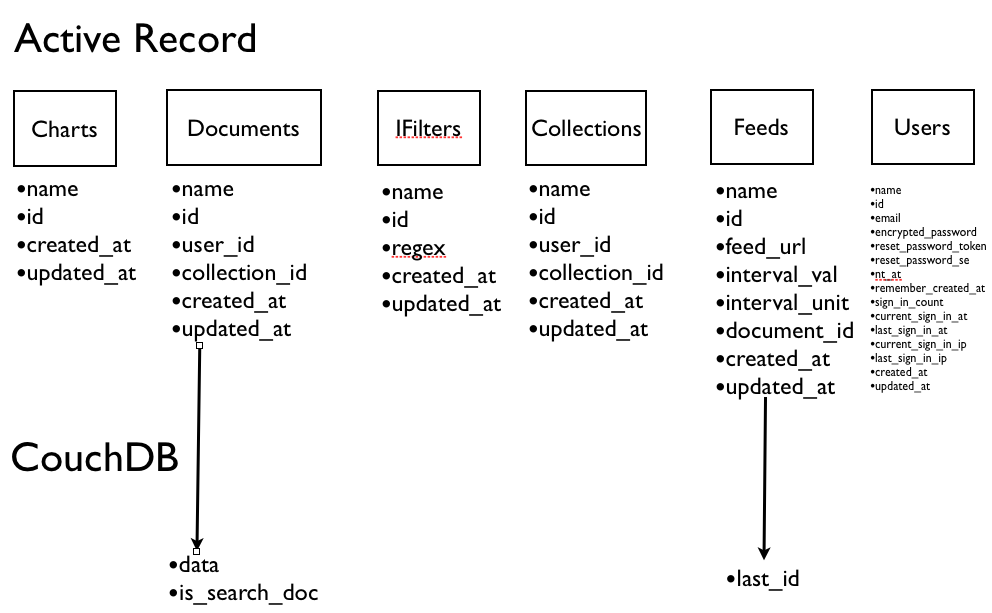
\includegraphics[width=120mm]{images/hatch_db_hybrid}
	\caption{The Hatch relational - non-relational database hybrid} 
	\label{hatch_db_hybrid}
	\end{center}
\end{figure}

The result is a relation - non-relational database hybrid. Hatch uses traditional 
relational database columns when the columns are ubiquitous, and can add columns to
a database entity (called scaffold) on the fly using CouchDB. For example, we create
a scaffold called Documents. Document always have a name, id, and collection/folder
they belong to. But, documents may have a data section, or they may not. That
data section may have infinite columns and rows of data, that would match the flat 
file they came from (like an Excel file). Or document may have any other data that
can be stored in JSON format. It is up to the Hatch interface, not database, to 
decide. And by allowing the interface to decide the structure and fields of data, Hatch
is by extension allowing the user to decide how to format data.

\pagebreak

\begin{figure}[h]
	\begin{center}
	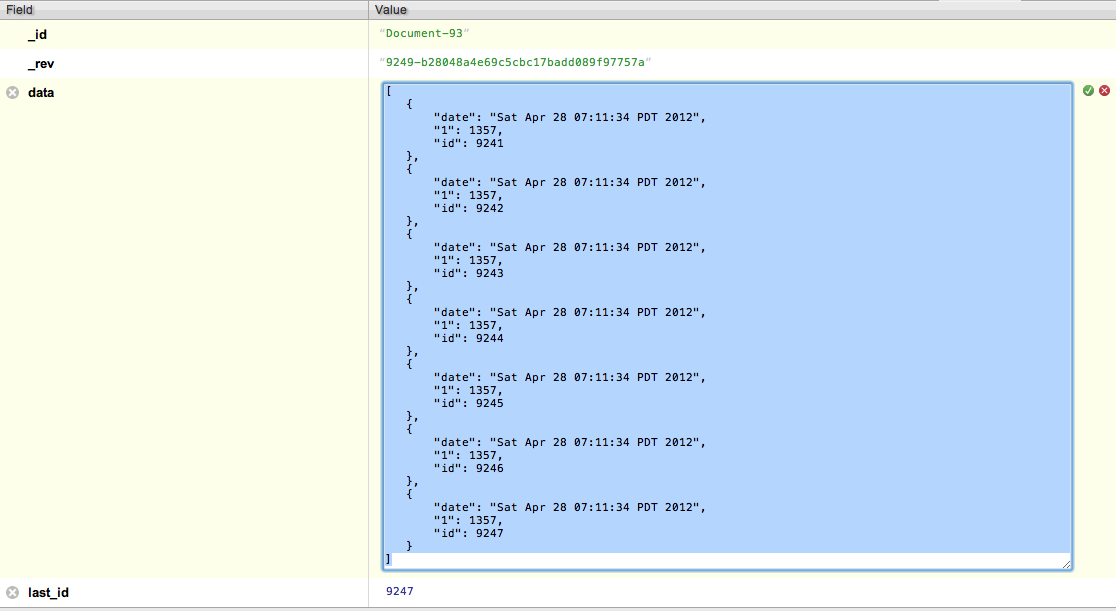
\includegraphics[width=120mm]{images/couchdb_json_ex}
	\caption{Typical representation of document data in CouchDB / JSON} 
	\label{couchdb_json_ex}
	\end{center}
\end{figure}

Most Rails applications that use CouchDB completely replace Active Record with some
library's version of it, like \textbf{couchrest's Active Model}. But if you replace
Active Record, you lose tons of support for libraries that lots of Rails developers
make, like pagination. 

Hatch gets around this by using its database hybrid, using a Ruby library called
\textbf{stuffing}. Stuffing is a link that ties Rails Active Record records with
CouchDB documents. It allows for rapid prototyping in development, and is a nice, modest
alternative to ripping out the guts of Active Record. Since the base model for 
database scaffolds are still Active Record, the huge amount of Rails Active Record based
libraries still work.


